\chapter{Définitions générales sur les courbes elliptiques}
\begin{center}
    Dans ce chapitre, on donne d'abord la définition générale d'une courbe elliptique. On fait
    le lien entre cette définition et la définition qui utilise une forme simplifiée de
    l'équation générale. On propose également un lemme qui permet de caractériser simplement les courbes
    non-lisses. Finalement, on donne la définition d'un point rationnel d'une courbe
    elliptique.
\end{center}

\section{Définition générale}

La définition générale d'une courbe elliptique est la suivante
\begin{definition}
    Soient $K$ un corps, $\overline{K}$ sa cloture algébrique, et $K^{*}$ son groupe
    multiplicatif. Une courbe elliptique sur $K$ est une cubique, non singulière,
    définie comme l'ensemble des solutions du plan projectif $\mathbb{P}_{2}(\overline{K})$ de
    l'équation de Weierstrass homogène suivante:

\begin{align}
\label{eq:geneEll}
E: Y^2Z+a_1XYZ+a_3YZ^2 = X^3 +a_2X^2Z+a_4XZ^2+a_6Z^3
,\end{align}

avec $a_1,a_2,a_3,a_4$ et $a_6$ dans $K$.
\end{definition}
Le terme non singulière, signifie que la courbe est lisse. Ce qui veut dire que si on écrit
l'équation précédente sous la forme d'une équation homogène $F(X,Y,Z)=0$, alors les dérivées
partielles de $F$ ne doivent pas s'annuler simultanément en un point de la courbe.

Autrement dit, il n'existe pas de point $P = \left[ x_0,y_0,z_0 \right] \in \mathbb{P}^2$ tel
que, en posant
\[
F(x,y,z) = y^2z+a_1xyz+a_3yz^2 - x^3-a_2x^2z-a_4xz^2-a_6Z^3
,\] 
on ait
\[
F(x_0,y_0,z_0)=\frac{\partial{F}}{\partial{x}}(x_0,y_0,z_0) =
\frac{\partial{F}}{\partial{y}}(x_0,y_0,z_0) =
\frac{\partial{F}}{\partial{z}}(x_0,y_0,z_0) = 0
.\] 

Dans une courbe elliptique la droite à l'infini ne contient qu'un seul élément, on le nomme
point à l'infini et on le note $O = [0,1,0]$.

Par la suite nous utiliserons la plupart du temps la représentation affine de
l'équation de Weierstrass:

\begin{align}
    \label{eq:geneAff}
E : y^2 + a_1xy + a_3 = x^3 +a_2x^2+a_4x+a_6
.\end{align}
avec les $a_{i} \in K$. 

Pour $Z \neq 0$, un point $[x,y,z] \in \mathbb{P}_{2}$ solution de l'équation
\eqref{eq:geneEll} correspond à un point $(x,y) \in \overline{K}^2$ solution de
l'équation \eqref{eq:geneAff} avec $(x,y)=(\frac{X}{Z},\frac{Y}{Z})$.

L'ensemble des solutions de l'équation \eqref{eq:geneEll} correspond à l'union entre les
solutions de l'équation \eqref{eq:geneAff} et du point $O$.

Ce qui revient à écrire que

\begin{align*}
    E &= \left\{ (X,Y,Z) \in \overline{K}^2 \times \overline{K}^{*} \mid F(X,Y,Z) = 0 \right\}  \cup
\{O\} \\
&= \left\{ (x,y) \in \overline{K}^2 \mid f(x,y) = 0 \right\} \cup \{O\}
.\end{align*}

On peut, par un double changement linéaire de variable, obtenir l'équation courte de Weierstrass
pour des corps de caractéristique différente de 2 et 3.

En effet, l'idée est d'effectuer un changement pour la variable $y$ qui nous permet
d'obtenir un polynôme de la forme
\[
E' :\quad Y^2 = X^3 + k_1X^2 + k_2X + k_3
,\] 
où les $k_{i}$ sont des constantes divisées par un multiple de deux.

Ensuite, en effectuant un changement de variable pour $x$, on se ramène au polynôme qui nous
intéresse à savoir 
\begin{align}
    \label{eq:geneWei}
E'' :\quad Y^2 = X^3 + k_1X + k_2
.\end{align}
où les $k_{i}$ cette fois-ci sont divisés par des multiples de 2 et 3.

On peut ainsi, démontrer que $K$ étant de caractéristique distincte de 2 et 3, une courbe
lisse d'équation \eqref{eq:geneEll} est "isomorphe sur $K$" à une courbe de la forme
\eqref{eq:geneWei} pour laquelle le discriminant du polynôme homogène
associé soit non nul.  La définition que l'on va utiliser n'est donc pas restrictive.

% \section{Définition appliqué à la cryptographie}

C'est pourquoi, dans la totalité de ce qui suit la lettre $K$ désignera un corps de caractéristique $0$ ou un
corps fini de caractéristique distincte de $2$ et $3$. Autrement dit, on peut voir $K$
comme étant l'un des corps commutatifs suivant $\Q,\ \R,\ \C$ ou $\mathbb{F}_{q}$.

On va plutôt se servir de la définition suivante qui est celle qui nous intéresse en
vue de construire le groupe des points rationnels d'une courbe elliptique appliqué à la cryptographie.

\begin{definition}
    \label{def:ell}
    Une courbe elliptique définie sur $K$ est une courbe projective plane d'équation
    \begin{align}
        \label{eq:ell}
    y^2z=x^3+axz^3+bz^2
    .\end{align}
    où $a$ et $b$ sont des éléments de $K$ vérifiant la condition
    \begin{align}
        \label{eq:delta}
    4a^3+27b^2\neq 0
    .\end{align}
\end{definition}

\begin{remarque}
On dit que la courbe elliptique d'équation \ref{eq:ell} est définie sur $K$ pour préciser
que $a$ et $b$ sont dans $K$. Ceci pour $a$ et $b$ vérifiant la condition \eqref{eq:delta} 
\end{remarque}

On a donc le polynôme $F(X,Y,Z)$ dans l'anneau de polynôme $K[X,Y,Z]$ associé à la courbe et
$E$ est défini par l'ensemble des solutions de l'équation 
\[
E:\quad F(X,Y,Z) = Y^2Z-\(X^3+aXZ^3+bZ^2\) = 0
.\] 

\begin{remarque}
    \begin{enumerate}
        \item 
Les points du plan projectif qui satisfont cette équation sont appelés l'ensemble des zéros
de $F$ dans $\overline{K}$, ou plus simplement zéro de $F$. Cet ensemble est ce que l'on
entend par courbe projective plane d'équation \eqref{eq:ell}. 
        \item Si $\Delta<0$, alors il
            admet une racine réelle et deux racines complexes et on obtient des courbe de la
            forme suivante
            \begin{figure}[h]
                \centering
                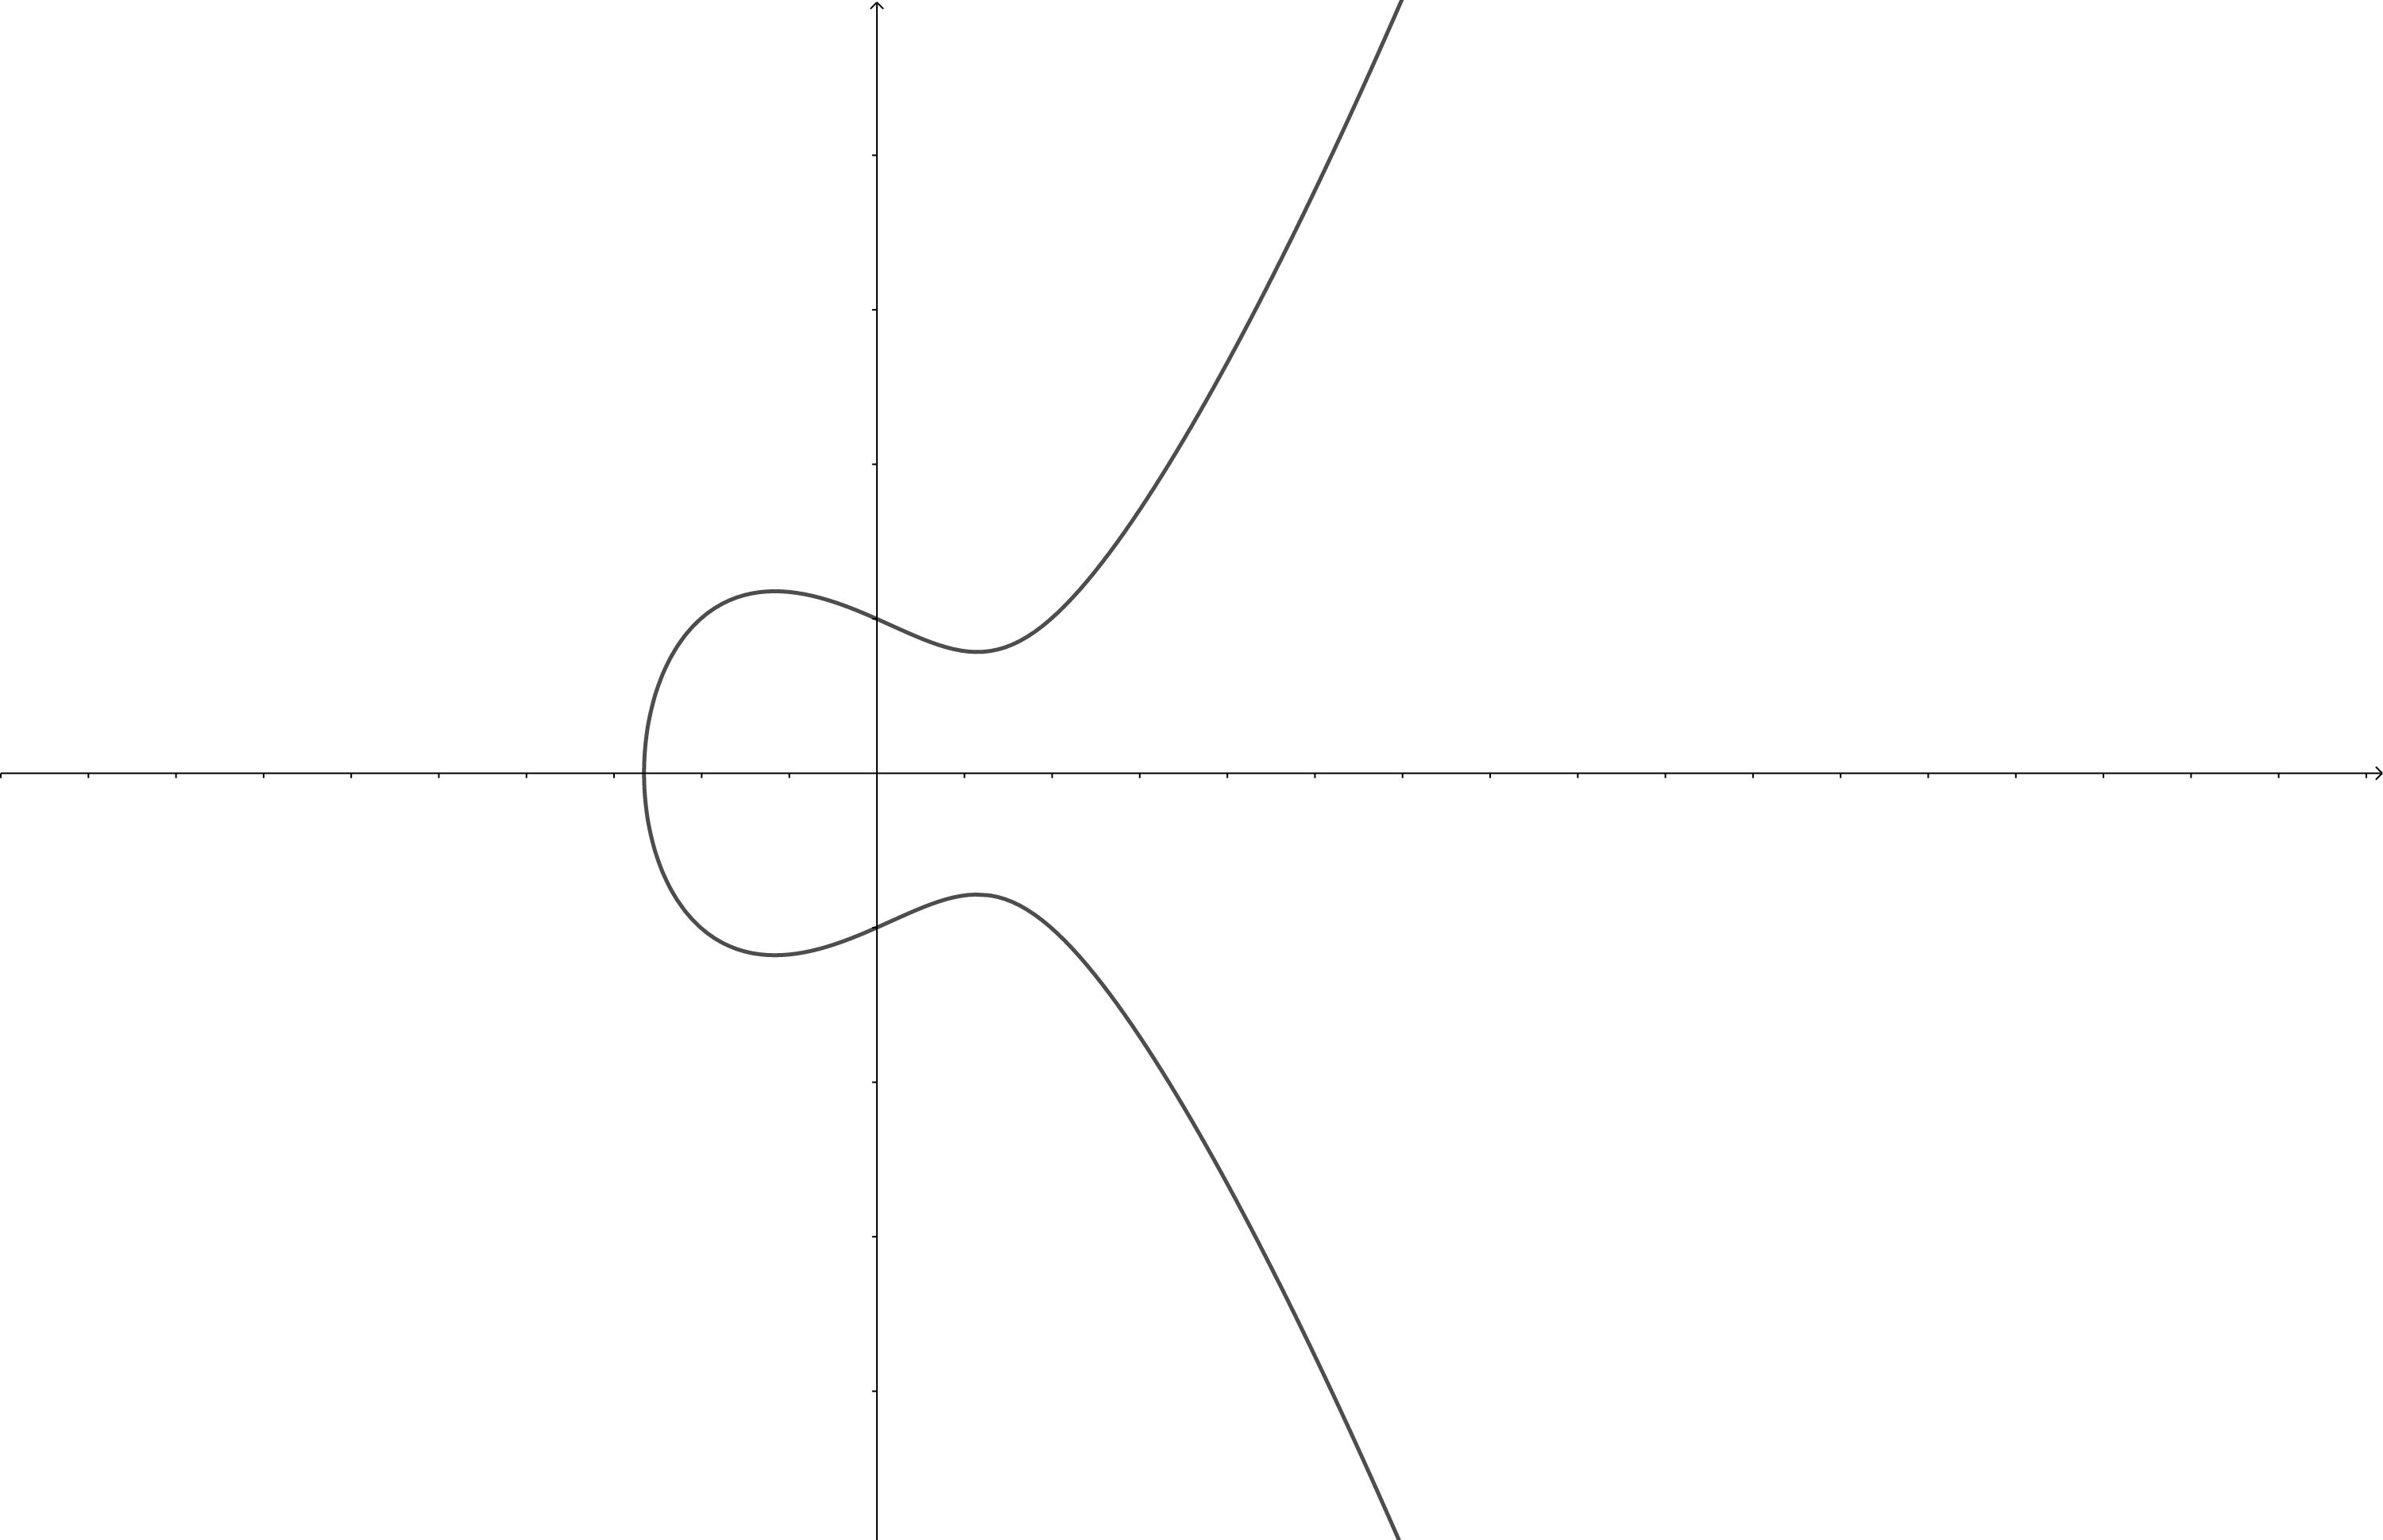
\includegraphics[width=0.4\textwidth]{deltaNeg}
                \caption{Courbe elliptique d'équation $y^2 = x^3 - x + 1$}
                \label{fig:deltaNeg}
            \end{figure}
        \item Si $\Delta > 0$, on a trois racines réelles distinctes et donc des courbes
            elliptiques de la forme suivante
            \begin{figure}[h]
                \centering
                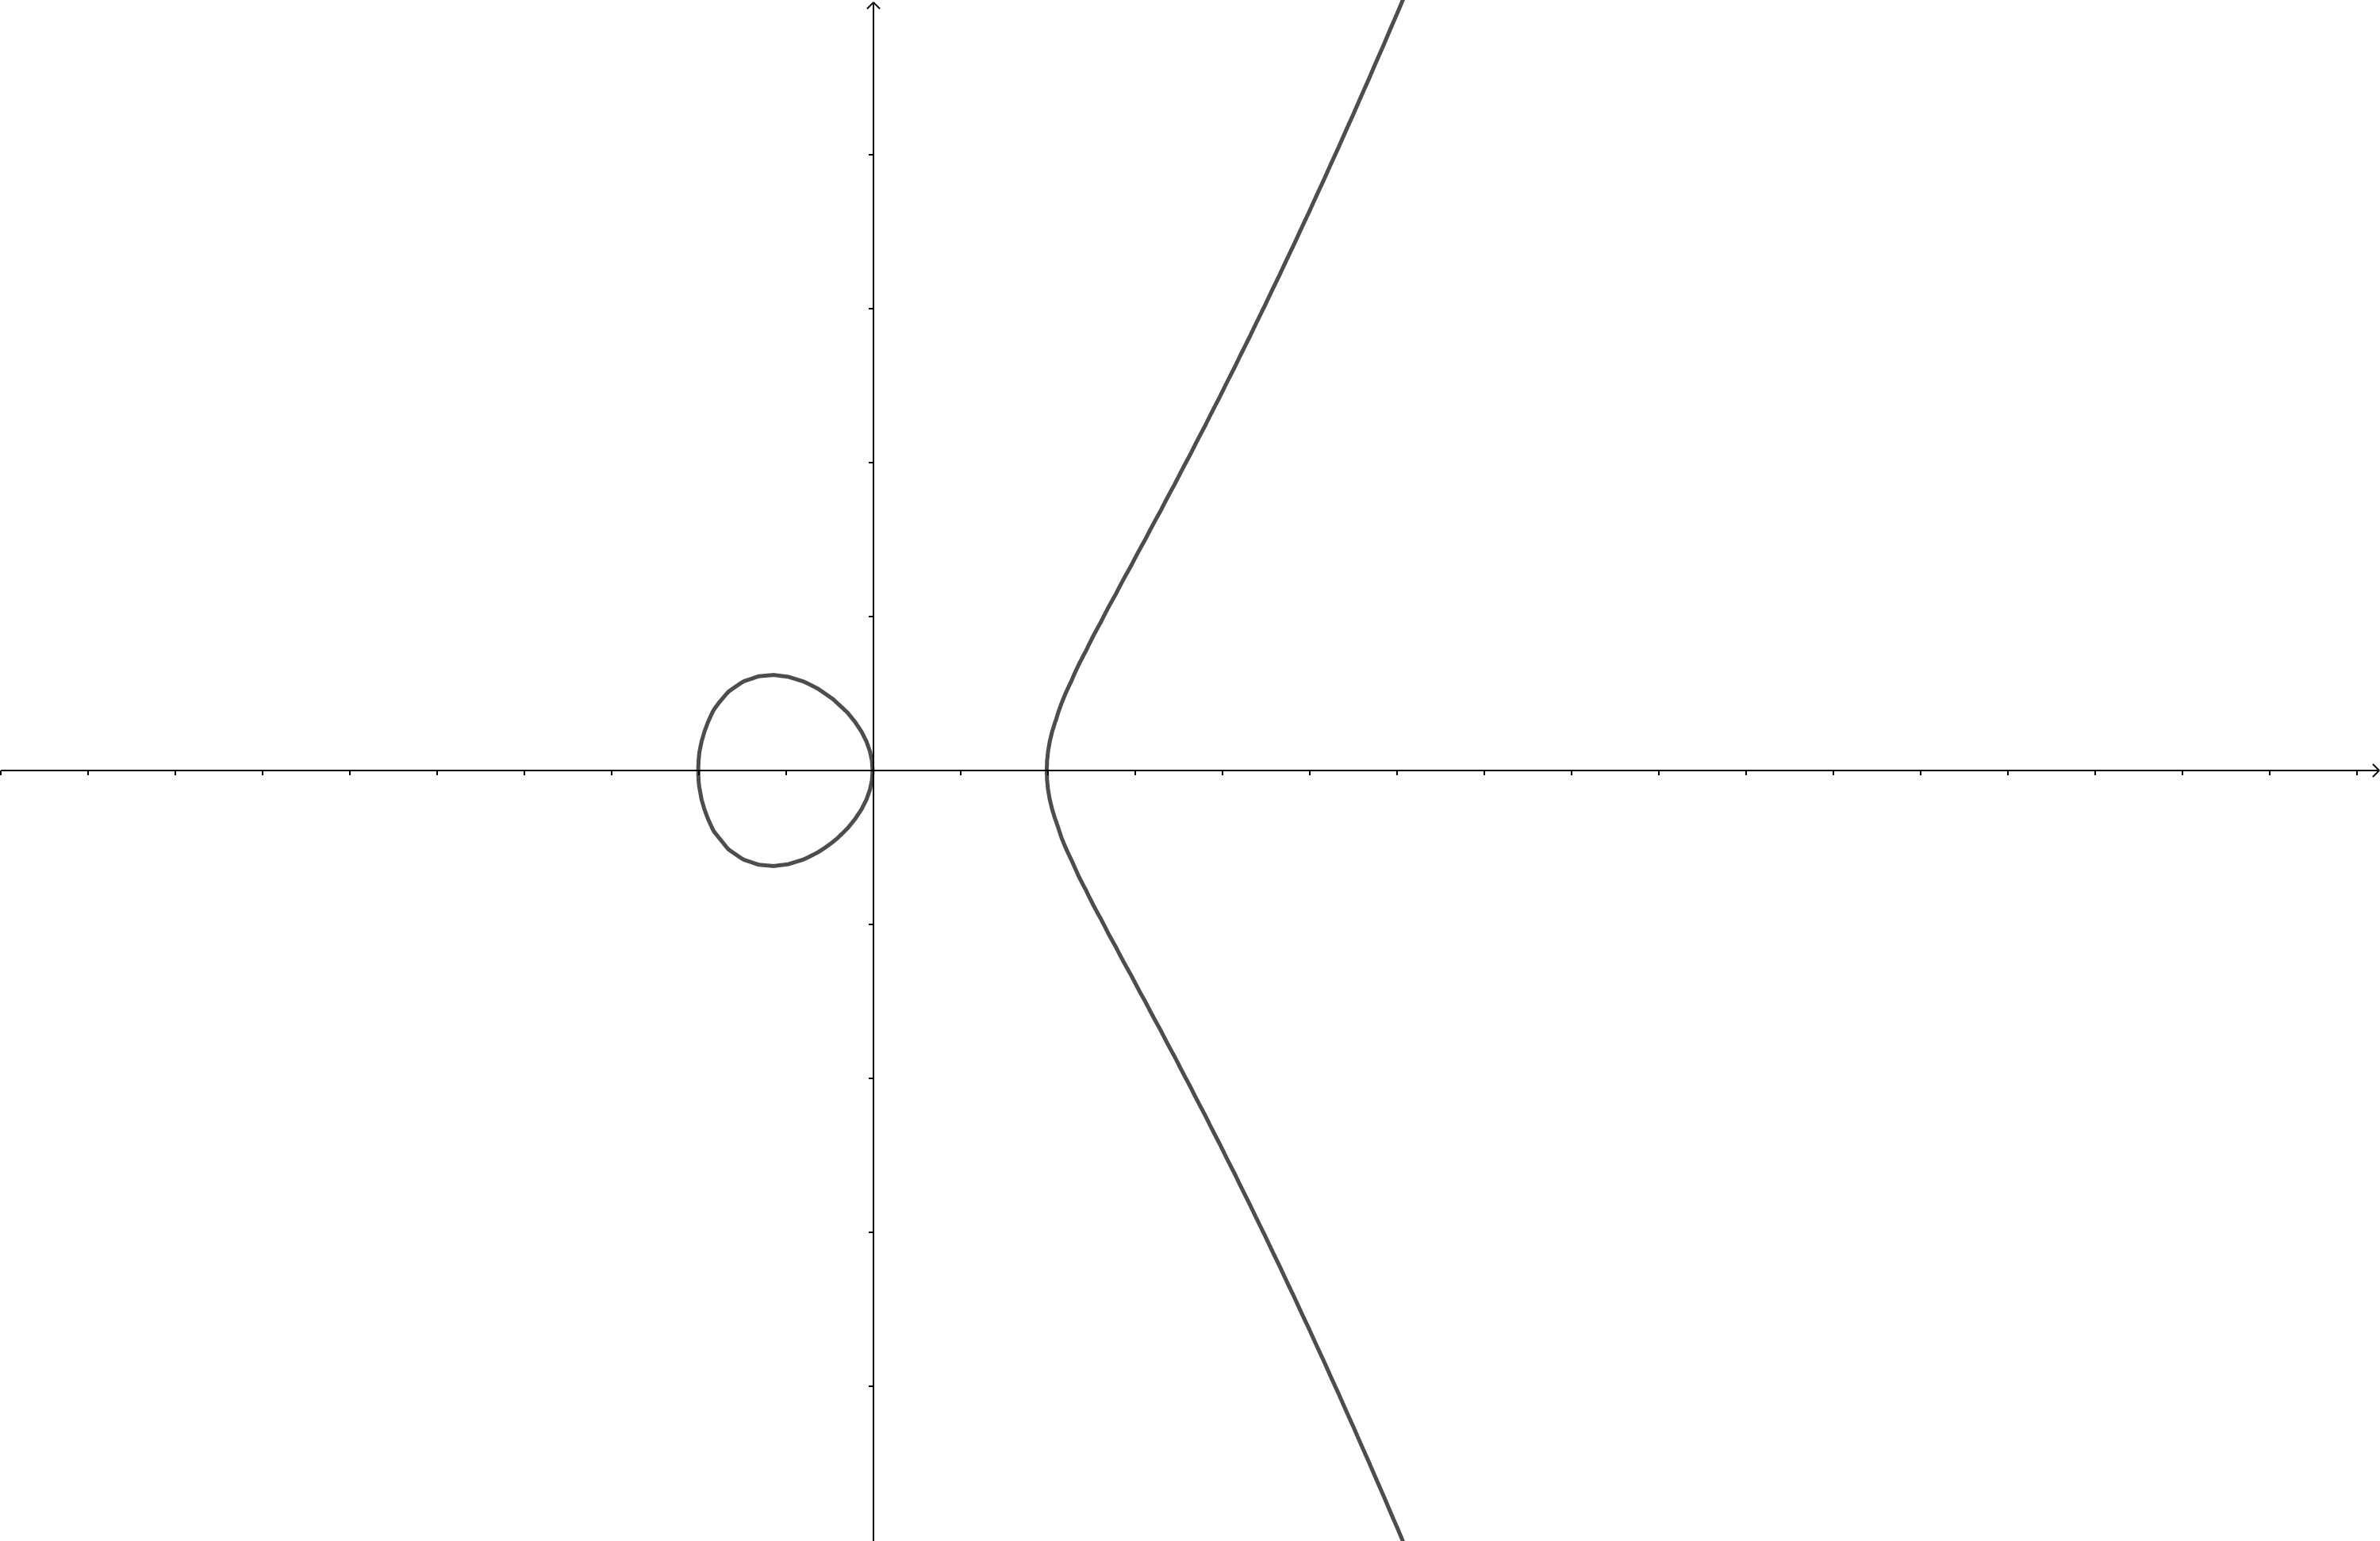
\includegraphics[width=0.4\textwidth]{deltaPos}
                \caption{Courbe elliptique d'équation $y^2 = x^3 - x$.}
                \label{fig:deltaPos}
            \end{figure}

        \item Si $\Delta = 0$ alors la courbe n'est pas elliptique et on obtient un point
            singulier.
            \begin{figure}[h]
                \centering
                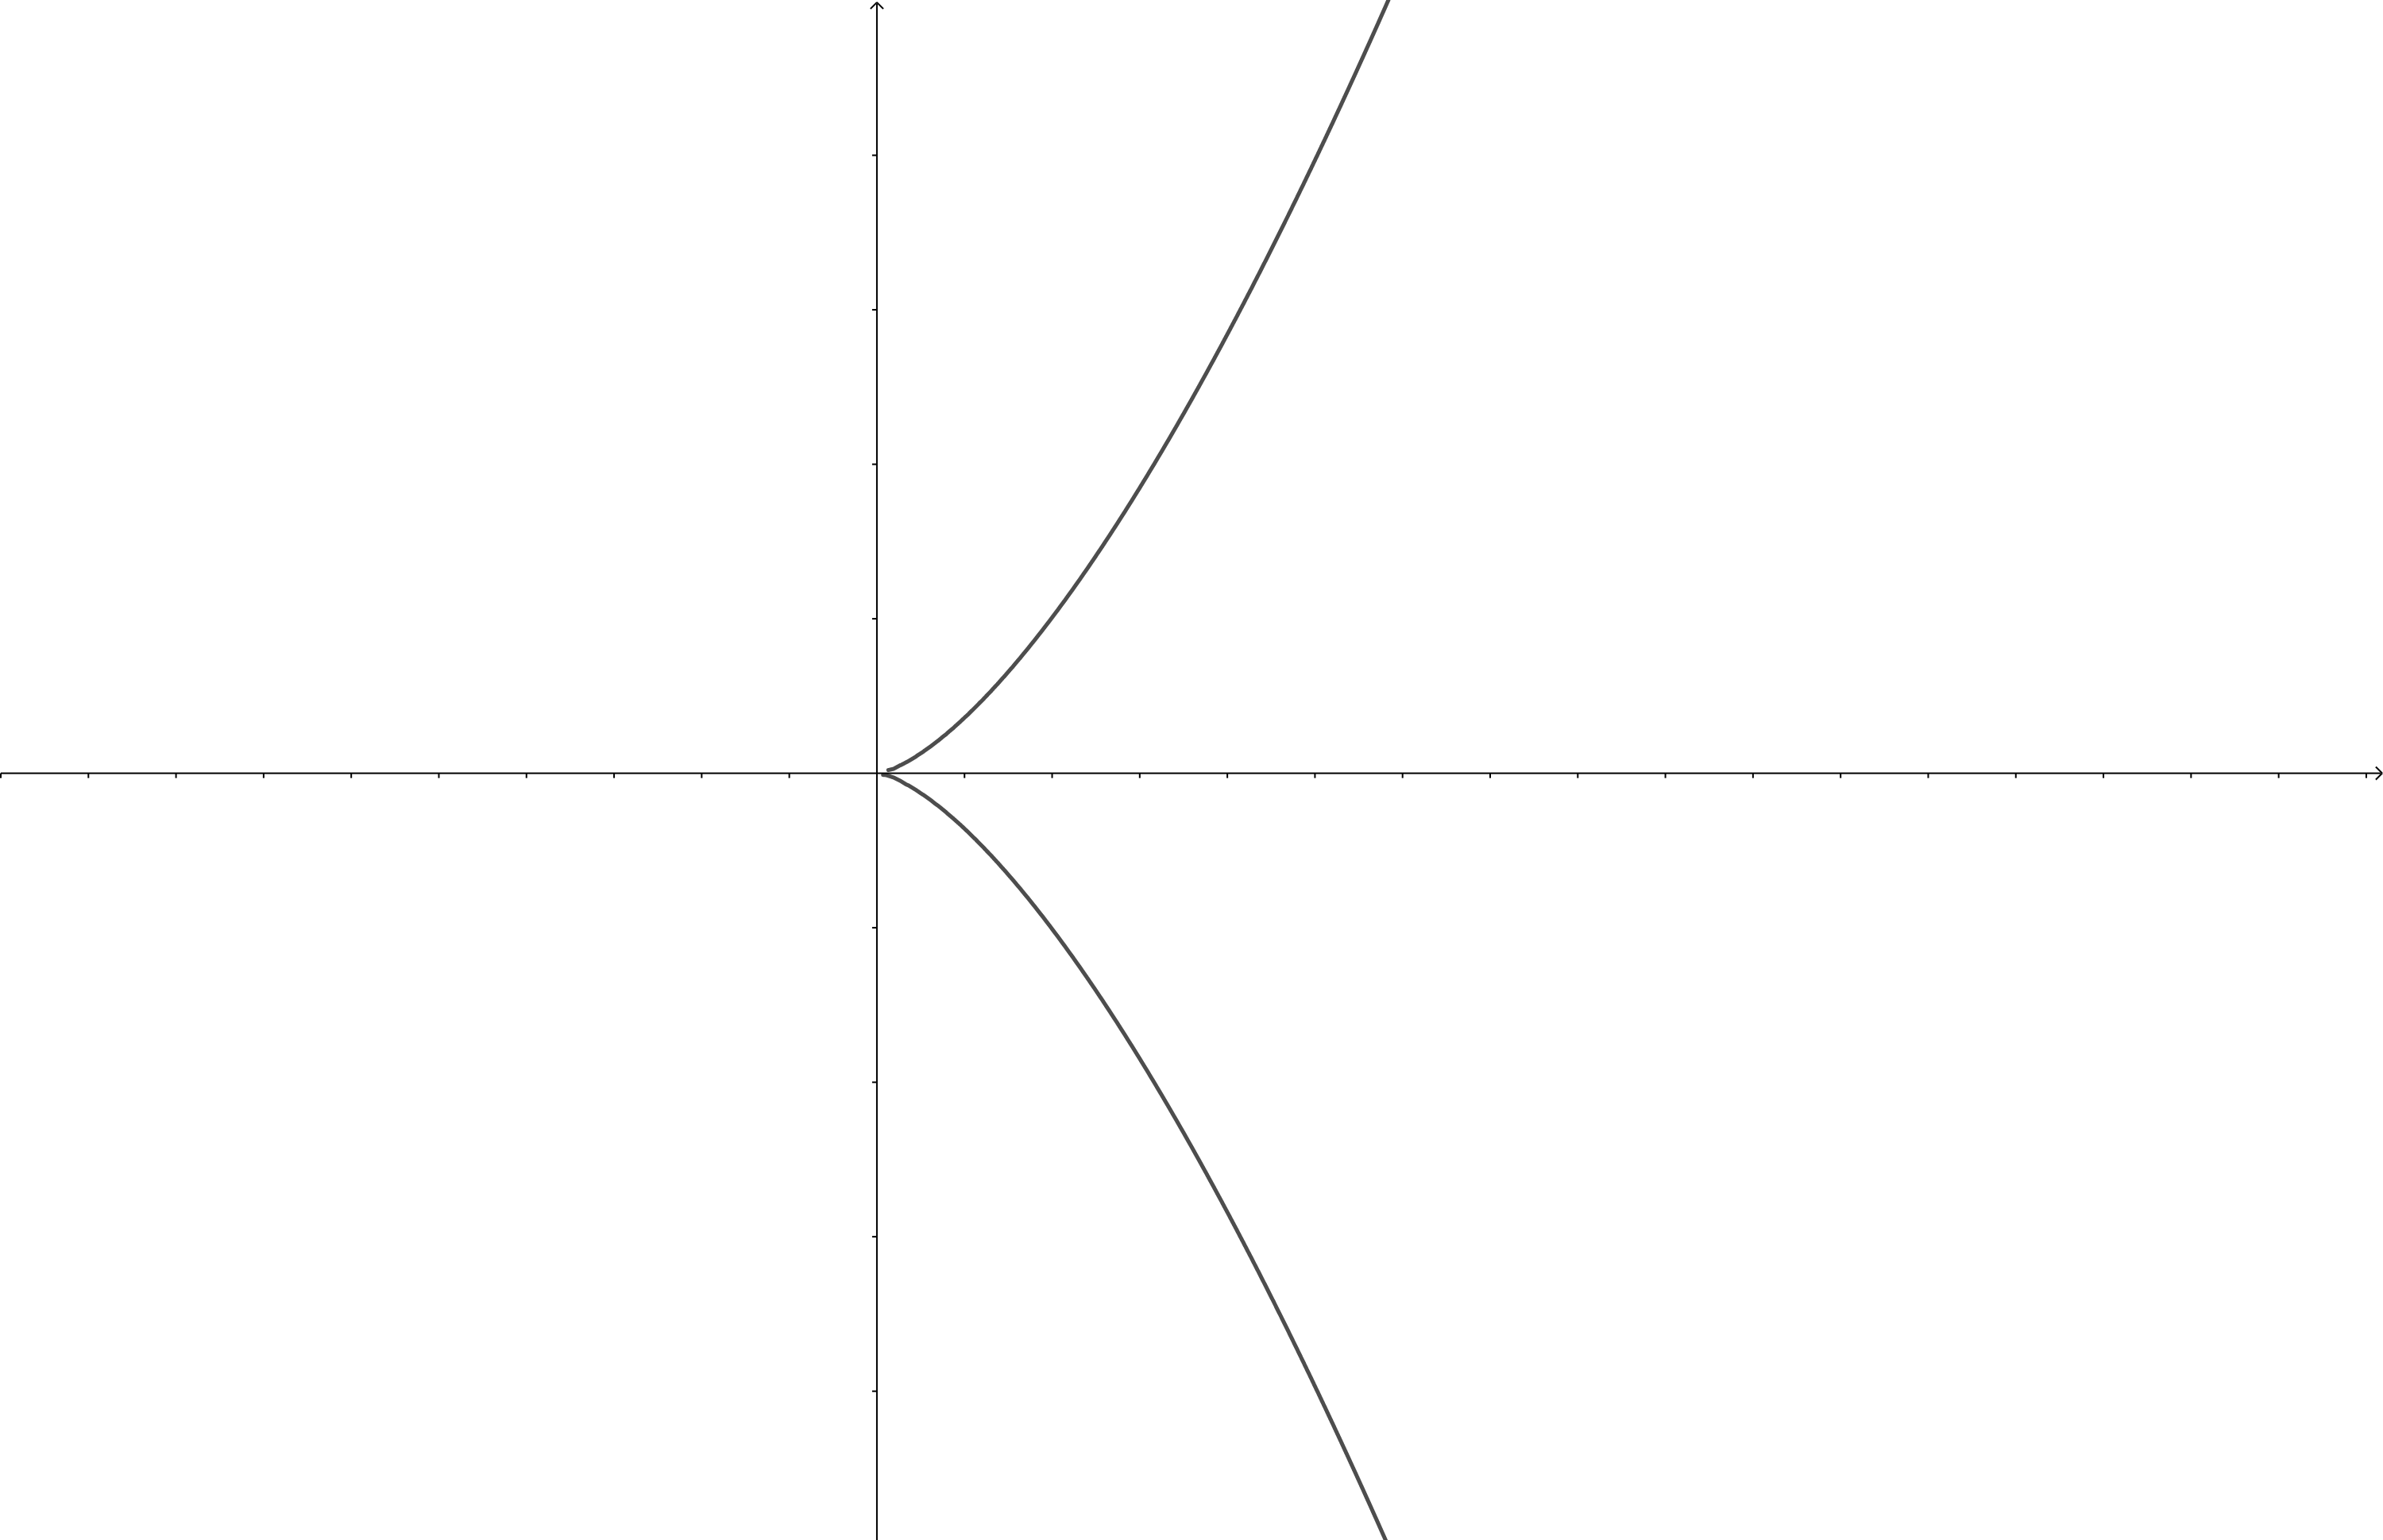
\includegraphics[width=0.4\textwidth]{deltaNul}
                \caption{Courbe elliptique d'équation $y^2 = x^3$.}
                \label{fig:deltaNul}
            \end{figure}
    \end{enumerate}
\end{remarque}

Comme on vient de le voir, il est possible de se ramener à l'étude
des solutions de l'équation
polynômiale $f(x,y) = 0$ dans le plan affine. Ainsi la condition \eqref{eq:delta}
signifie que les racines dans $\overline{K}$ du polynôme
\[
f(x,y) = y^2 - \(x^3 + ax + b\)
,\] 
sont simples et le lemme suivant nous fournit un critère simple pour obtenir une courbe
lisse. Ce qui nous permet d'éviter les courbes avec un point de multiplicité double qui nous
fait perdre l'unicité de la tangente.
\begin{figure}[h]
    \centering
    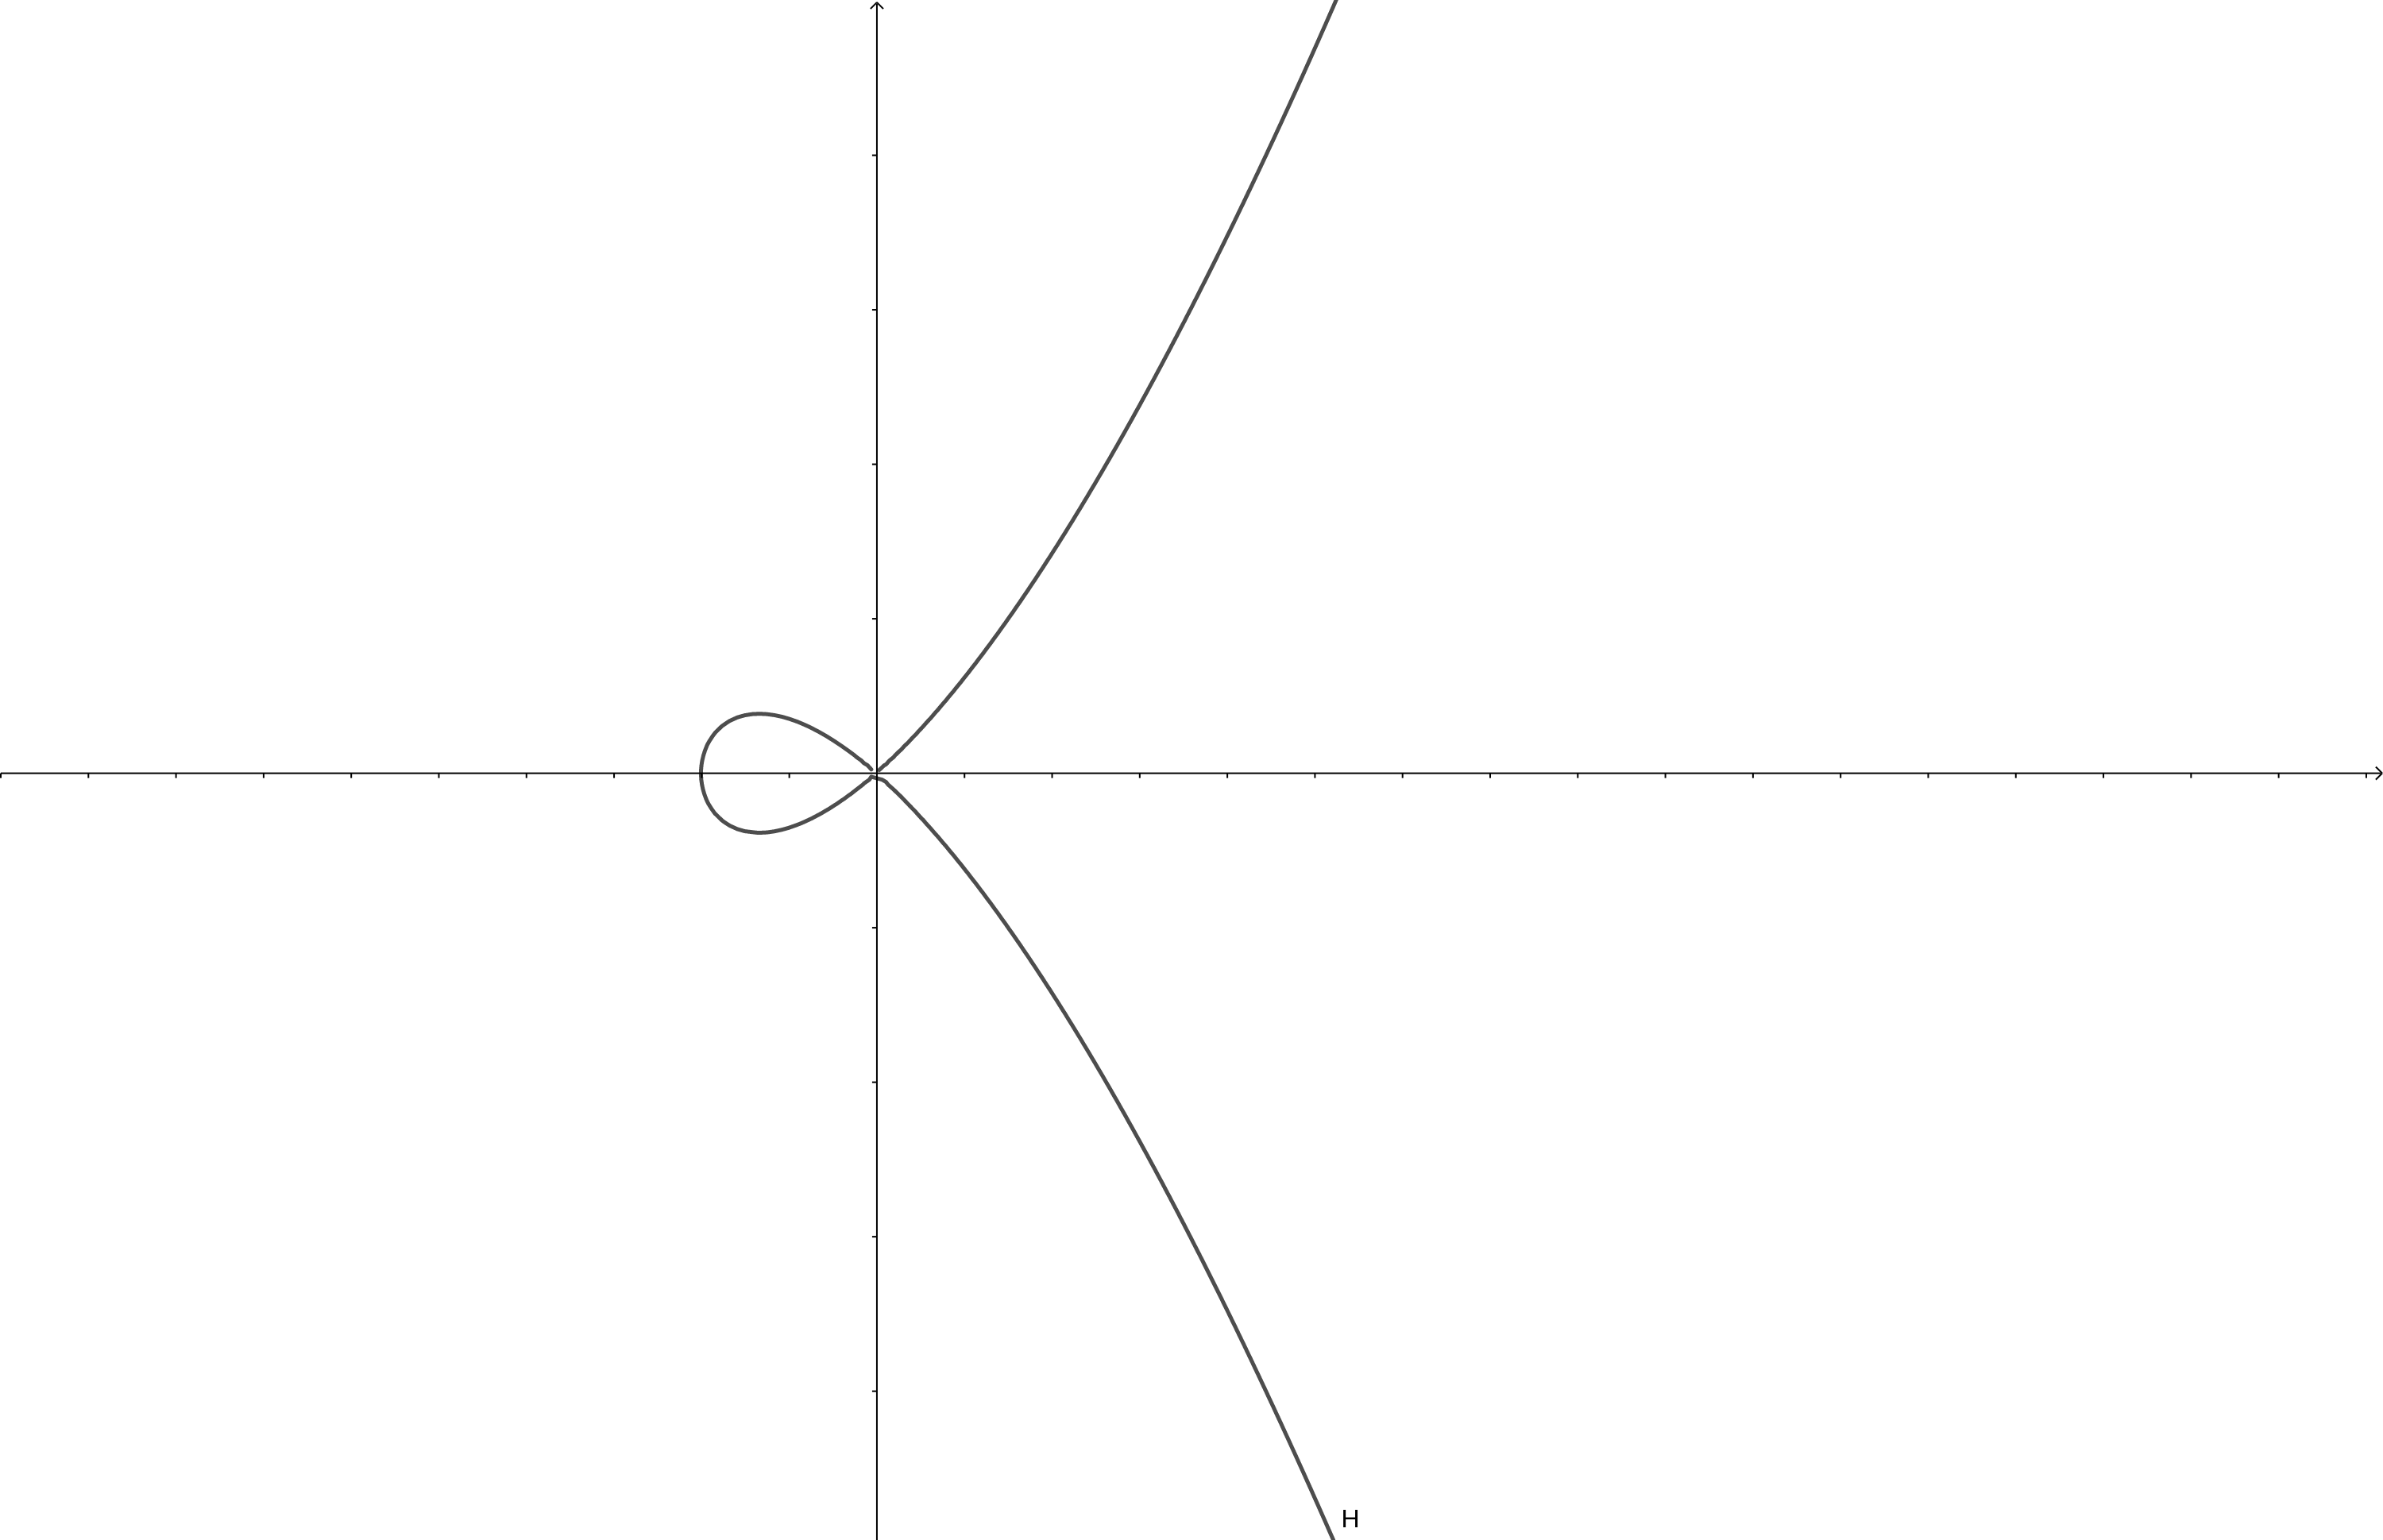
\includegraphics[width=0.5\textwidth]{courbeSing}
    \caption{Courbes d'équation $y^2 = x^3 + x^2$ admettant un point double.}
    \label{fig:courbeSing}
\end{figure}

\begin{lemme}
    \label{lem:lemme1}
    Le discriminant de $f\ : x^3 + ax + b$ est $\Delta = -(4a^3 + 27b^2)$. En particulier, les racines de $f$ sont simples, si et seulement si $\Delta \neq 0$.
\end{lemme}

Pour démontrer ce lemme, on utilise la proposition que nous admettrons, qui est la suivante:
\begin{proposition}
    \label{prop:discriminant}
    Soit $g$ un polynôme unitaire à coefficients dans $K$ de degré $n \ge 1$. Soient
    $\alpha_1,\ldots,\alpha_{n}$ ses racines dans $\overline{K}$ comptées avec
    multiplicités. Le discriminant $\Delta$ de $g$ est défini par l'égalité
    \[
    \Delta = \prod_{i<j}^{} \left( \alpha_{i} - \alpha_{j} \right) ^2 
    .\] 
    C'est un élément de $K$.
\end{proposition}

\begin{demonstration}[Lemme]
    Montrons tout d'abord que le discriminant de $f$ est $\Delta= -(4a^3 + 27b^2)$.

    Soit $\Delta$ le discriminant de $f$. Soient $\alpha, \beta, \gamma $ les racines de $f$ dans $\overline{K}$ et $f'$ le polynôme dérivé de $f$.

    À l'aide de la proposition \ref{prop:discriminant}, on veut montrer que le discriminant est de la forme
    suivante: 
    \begin{align*}
        \Delta &= (-1) ( \alpha - \beta )^2 ( \alpha - \gamma )^2 ( \beta - \gamma )^2 \\
          &= - f(\alpha)'f(\beta )'f(\gamma)'
    .\end{align*}

    Vérifions que c'est bien le cas.

    D'aprés le théorème d'Alembert-Gauss comme $f \in \overline{K}$, on dispose de la
    forme scindée de $f$.
    \[
        f = \left( X - \alpha \right) \left( X - \beta \right) \left( X - \gamma \right) 
    .\] 
    En dérivant $f$ sous cette forme on obtient :
    \begin{align*}
        f &= ( X - \alpha ) \left( ( X - \beta ) ( X - \gamma ) \right)'  + ( X - \beta ) ( X - \gamma )\\
          &= ( X - \alpha ) \left( ( X - \beta ) + ( X - \gamma ) \right) + ( X - \beta ) ( X - \gamma ) 
    .\end{align*}

    Donc  
\[
f' = ( X - \alpha ) ( X - \beta ) + ( X - \alpha ) ( X - \gamma ) + ( X - \beta ) ( X - \gamma )
.\] 

On a alors successivement : 
\[
    f(\alpha)' = ( \alpha - \beta) ( \alpha - \gamma )
,\] 
\[
f(\beta )' = ( \beta - \alpha) ( \beta - \gamma)
,\] 
et
\[
f(\gamma)' = ( \gamma - \alpha) ( \gamma - \beta)
.\] 

En multipliant ces trois expressions, on obtient :
\begin{align*}
    f(\alpha)' f(\beta )' f(\gamma)' &= ( \alpha - \beta ) ( \alpha - \gamma ) ( \beta - \alpha ) ( \beta - \gamma) ( \gamma - \alpha ) ( \gamma - \beta ) \\
&= \left( X - \alpha \right) \left( \alpha - \gamma \right) \left( -1 \right) \left( \alpha - \beta  \right) \left( \beta - \gamma \right) \left( -1 \right) \left( \alpha - \gamma \right) \left( -1 \right) \left( \beta - \gamma \right) \\
&= \left( -1 \right) ^3 \left( \alpha - \beta  \right) ^2 \left( \alpha - \gamma  \right) ^2 \left( \beta - \gamma \right) ^2\\
 &= - \Delta
.\end{align*}

Et donc 

\[
\Delta = - f'(\alpha) f'(\beta ) f'(\gamma)
.\] 

En partant de la forme $f : x^3 + ax + b$, on remarque que $f' : 3x^2 + a$. Par suite on obtient,
\begin{align*}
    \Delta &= - f'(\alpha) f'(\beta ) f'(\gamma) \\
      &= - \left( 3 \alpha^2 + a \right) \left( 3 \beta^2 + a \right) \left( 3 \gamma^2 + a \right) 
.\end{align*}
Ce qui donne :
\begin{align*}
    \Delta  &= - \left( ( 9 \alpha^2 \beta^2 + 3a ( \alpha^2 + \beta^2 ) + a^2 ) ( 3 \gamma^2 + a ) \right)  \\
       &= - \left( 27 \left( \alpha \beta \gamma \right)^2  + 9a \left( \alpha^2 \beta^2 + \alpha^2 \gamma^2 + \beta^2 \gamma^2 \right) + 3a^2 \left( \alpha^2 + \beta^2 + \gamma^2 \right) + a^3 \right) 
.\end{align*}
On peut écrire
\[
\alpha^2 + \beta^2 + \gamma^2 = \left( \alpha + \beta + \gamma \right)^2 - 2 \left( \alpha \beta + \alpha \gamma + \beta \gamma \right)
,\] 
\[
\alpha^2 \beta^2 + \alpha^2 \gamma^2 + \beta^2 \gamma^2 = \left( \alpha \beta + \alpha \gamma + \beta \gamma \right)^2 - 2\alpha \beta \gamma \left( \alpha + \beta + \gamma \right)
.\] 
Donc d'après les relations entre coefficients et racines (i.e relation de Viète), pour un polynôme de la forme $ax^3 + bx^2 + cx + d$, on a :
\[
\alpha + \beta + \gamma = - \frac{b}{a}
,\] 
\[
\alpha \beta + \alpha \gamma + \beta \gamma = \frac{c}{a}
,\] 
\[
\alpha \beta \gamma = - \frac{d}{a}
.\] 
Ici dans $f$ on a $a = 1$, $b = 0$, $c = a$ et $d = b$.

D'où,
\[
\alpha + \beta + \gamma = 0 \text{, } \alpha \beta + \alpha \gamma + \beta \gamma = a \text{ et } \alpha \beta \gamma = - b
.\] 
Ce qui donne : 
\begin{align*}
    \alpha^2 + \beta^2 + \gamma^2 &= 0^2 - 2a = -2a \\
    \alpha^2 \beta^2 + \alpha^2 \gamma^2 + \beta^2 \gamma^2 &= a^2 + 2b \times 0
.\end{align*}

Donc le discriminant vaut :
\begin{align*}
    \Delta &= - \left( 27b^2 + 9a^3 - 6a^3 + a^3  \right) \\
        &= - \left( 4a^3 + 27b^2  \right)
.\end{align*}

Montrons maitenant que les racines de $f$ sont simples, si et seulement si, $\Delta \neq 0$

Raisonnons par contraposition et montrons que les racines de $f$ sont multiples, si et
seulement si, $\Delta = 0$. 

Supposons que $\Delta = 0$. On a alors :
 \begin{align*}
     - \left( 4a^3 + 27^2 \right) = 0 &\iff - f(\alpha)' f(\beta )' f(\gamma)' = 0 \\
                                      & \iff \left( f(\alpha)' = 0 \right) \ou \left( f(\beta )' = 0 \right) \ou \left( f(\gamma)' = 0 \right) \\
                                      &\iff \alpha \text{ ou } \beta \text{ ou } \gamma \text{ est une racine multiple}
.\end{align*}

D'où le résultat.
\end{demonstration}

\section{Points rationnels d'une courbe elliptique}

Soit $L$ une extension de $K$ dans $\overline{K}$.

\begin{definition}
    Soit $P=\left[ x,y,z \right] $ un point de $\mathbb{P}^2$. On dit que $P$ est rationnel sur $L$ s'il existe $\lambda \in \overline{K}^{*}$ tel que $\lambda x$, $\lambda y$ et $\lambda z$ soient dans $L$. On note $\mathbb{P}^2(L)$ l'ensemble des points de $\mathbb{P}^2$ rationnels sur $L$.

\end{definition}

D'aprés la définition ci-dessus, un point non nul $P$ est dans $\mathbb{P}_{2}(L)$, si sa classe est dans $L$. Autrement
dit, 
\[
\mathbb{P}_{2}(L)=\left\{ P \in \overline{K}^{3} \mid \exists \lambda \in \overline{K}^{*}, P =
\lambda P\right\} 
.\] 

Cela justifie la notation $\mathbb{P}^2 = \mathbb{P}^2(\overline{K})$.

\begin{remarque}
    Étant donné un point $[x_1,x_2,x_3] \in \mathbb{P}^2$, le fait qu'il soit rationnel sur $L$ n'implique pas que les $x_{i}$ soient dans $L$. Cela signifie qu'il existe $i$ tel que $x_{i}$ soit non nul, et que chaque $\frac{x_{j}}{x_{i}}$ appartienne à $L$.

    En effet, soit un point $P \in \mathbb{P}_{2}$ non nul. Si $P \in \mathbb{P}_{2}(L)$,
    comme il est non nul, il existe $x \neq 0$, et pour $\lambda = x$, on a $P =
    [1,\frac{y}{x},\frac{z}{x}]$ et on a bien $\frac{y}{x},\frac{z}{x} \in L$ et pourtant ce
    sont des variables indéterminées de $\overline{K}$.
\end{remarque}

Soit $E$ une courbe elliptique définie sur $K$ d'équation \eqref{eq:ell}.

\begin{definition}
    Un point de $E$ est dit rationnel sur $L$, ou encore $L$-rationnel, s'il appartient à $E \cap \mathbb{P}^2(L)$. On note $E(L)$ l'ensemble des points de $E$ rationnels sur $L$.
\end{definition}

Par définition, on a donc
\[
E = E(\overline{K})
.\] 

\begin{remarque}
    \begin{enumerate}
        \item  Lorsque le contexte est clair on parlera de point rationnel de la courbe pour
            parler des points $L$-rationnels.
        \item Le point $O$ est défini sur $K$ et par définition sur toute
            extension de $K$. Ainsi, si $L / K$ est une extension du corps $K$, $E$
            peut être considéré comme une courbe elliptique définie sur $K$ et $O$
            est encore le point à l'infini de $E / L$.

            On a,

            \[
            E(L) = \left\{ (x,y) \in L^2 \mid y^2 = x^3 + ax + b \right\} \cup \{O\}
            .\] 

            De même,
            \[
            E(\overline{K}) = \left\{ (x,y) \in \overline{K}^2 \mid y^2 = x^3 +
            ax + b \right\} \cup \{O\}
            .\] 

            Ce qui revient à dire que, si $K \subset L \subset \overline{K}$ alors $E(K)
            \subset E(L) \subset E(\overline{K})$.
    \end{enumerate}
\end{remarque}

\begin{exemple}
    \label{ex:F5}
    
    Soit la courbe $E$ définie sur $\mathbb{F}_{5}$ d'équation
    \[
    y^2 =x^3+x+1
    .\] 

    Cette courbe vérifie bien la condition \eqref{eq:delta}.
    
    En effet, on a $\Delta = -(4 \times 1^3 + 27 \times 1) = -31$.

    L'ensemble des points de la courbe est le suivant:
    \[
    E(\mathbb{F}_{5})= \left\{ (0,1),(0,4),(2,1),(2,4),(3,1),(3,4),(4,2),(4,3) \right\} \cup
    \left\{ O \right\} 
    .\] 

    Soit $\mathbb{F}_{25}$ le sous-corps de $\overline{\mathbb{F}}_{5}$ à 25
    éléments. On a
    \[
    \mathbb{F}_{25} = \mathbb{F}_{5}(\alpha) = \left\{ x + y\alpha \mid (x,y) \in
    \mathbb{F}_{5} \right\} 
    ,\] 
    où $\alpha \in \overline{\mathbb{F}}_{5}$ vérifie $\alpha^2 + \alpha + 1 = 0$.

    On constate que l'on a
    \[
    E(\mathbb{F}_{25}) = \{\left( 0 , \pm 1 \right) , \left( 2,\pm 1 \right) , \left( 3,\pm 1 \right)
    , \left( 4,\pm 2 \right), \left( 1+\alpha,\pm 2\alpha \right) , \left( 2+2\alpha, \pm
\left( 4 + \alpha \right)  \right) ,
    \] 
    \[
    \left( 2+3\alpha,\pm 2 \right) , \left( 4+2\alpha,\pm 2
\right), \left( 3\alpha, \pm \left( 2+\alpha \right)  \right) , \left( 1, \pm \left(
3+\alpha \right)  \right) ,
    \] 
    \[
    \left( 1 + 3 \alpha, \pm \left( 3+\alpha \right) \right) ,  \left( 3+2\alpha, \pm \left(
    3+\alpha \right)  \right)\}   \cup \{O\}
    .\] 
    
    .\end{align*}
\end{exemple}
